\documentclass[tikz,border=4pt]{standalone}
\usepackage{tikz}
\usetikzlibrary{arrows.meta}
\begin{document}
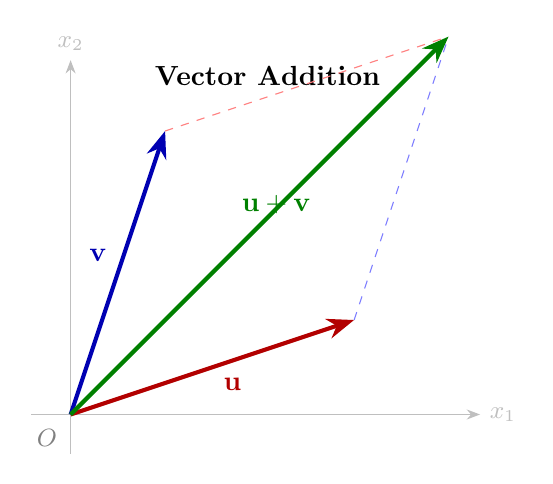
\begin{tikzpicture}[
    >=Stealth,
    axis/.style={->,gray!50},
    vec/.style={->,line width=1.5pt},
]
\node[font=\bfseries] at (2.5,4.3) {Vector Addition};

\draw[axis] (-0.5,0) -- (5.2,0) node[right,font=\small] {$x_1$};
\draw[axis] (0,-0.5) -- (0,4.5) node[above,font=\small] {$x_2$};

% Vector u: (3,1)
\draw[vec,red!70!black] (0,0) -- (3.6,1.2)
    node[midway,below right,font=\bfseries] {$\mathbf{u}$};

% Vector v: (1,3)
\draw[vec,blue!70!black] (0,0) -- (1.2,3.6)
    node[midway,above left,font=\bfseries] {$\mathbf{v}$};

% Parallelogram dashed
\draw[blue!50,dashed,thin] (3.6,1.2) -- (4.8,4.8);
\draw[red!50,dashed,thin] (1.2,3.6) -- (4.8,4.8);

% Result u+v: (4,4)
\draw[vec,green!50!black] (0,0) -- (4.8,4.8)
    node[midway,above,font=\bfseries,xshift=6pt] {$\mathbf{u}+\mathbf{v}$};

\node[font=\small,gray] at (-0.3,-0.3) {$O$};
\end{tikzpicture}
\end{document}
